
%% bare_jrnl_compsoc.tex
%% V1.3
%% 2007/01/11
%% by Michael Shell
%% See:
%% http://www.michaelshell.org/
%% for current contact information.
%%
%% This is a skeleton file demonstrating the use of IEEEtran.cls
%% (requires IEEEtran.cls version 1.7 or later) with an IEEE Computer
%% Society journal paper.
%%
%% Support sites:
%% http://www.michaelshell.org/tex/ieeetran/
%% http://www.ctan.org/tex-archive/macros/latex/contrib/IEEEtran/
%% and
%% http://www.ieee.org/

%%*************************************************************************
%% Legal Notice:
%% This code is offered as-is without any warranty either expressed or
%% implied; without even the implied warranty of MERCHANTABILITY or
%% FITNESS FOR A PARTICULAR PURPOSE! 
%% User assumes all risk.
%% In no event shall IEEE or any contributor to this code be liable for
%% any damages or losses, including, but not limited to, incidental,
%% consequential, or any other damages, resulting from the use or misuse
%% of any information contained here.
%%
%% All comments are the opinions of their respective authors and are not
%% necessarily endorsed by the IEEE.
%%
%% This work is distributed under the LaTeX Project Public License (LPPL)
%% ( http://www.latex-project.org/ ) version 1.3, and may be freely used,
%% distributed and modified. A copy of the LPPL, version 1.3, is included
%% in the base LaTeX documentation of all distributions of LaTeX released
%% 2003/12/01 or later.
%% Retain all contribution notices and credits.
%% ** Modified files should be clearly indicated as such, including  **
%% ** renaming them and changing author support contact information. **
%%
%% File list of work: IEEEtran.cls, IEEEtran_HOWTO.pdf, bare_adv.tex,
%%                    bare_conf.tex, bare_jrnl.tex, bare_jrnl_compsoc.tex
%%*************************************************************************

% *** Authors should verify (and, if needed, correct) their LaTeX system  ***
% *** with the testflow diagnostic prior to trusting their LaTeX platform ***
% *** with production work. IEEE's font choices can trigger bugs that do  ***
% *** not appear when using other class files.                            ***
% The testflow support page is at:
% http://www.michaelshell.org/tex/testflow/




% Note that the a4paper option is mainly intended so that authors in
% countries using A4 can easily print to A4 and see how their papers will
% look in print - the typesetting of the document will not typically be
% affected with changes in paper size (but the bottom and side margins will).
% Use the testflow package mentioned above to verify correct handling of
% both paper sizes by the user's LaTeX system.
%
% Also note that the "draftcls" or "draftclsnofoot", not "draft", option
% should be used if it is desired that the figures are to be displayed in
% draft mode.
%
% The Computer Society usually requires 10pt for submissions.
%\documentclass[journal,A4paper,epsfig]{IEEEtran}
%\documentclass[journal,letterpaper,epsfig]{IEEEtran}
%\documentclass[12pt,journal,letterpaper,peerreview,draftcls,onecolumn,doublespace,epsfig]{IEEEtran}

%\documentclass[journal,letterpaper,peerreview, epsfig]{IEEEtran}
\documentclass[10pt,journal,A4paper,compsoc,epsfig]{IEEEtran}
%
% If IEEEtran.cls has not been installed into the LaTeX system files,
% manually specify the path to it like:
% \documentclass[12pt,journal,compsoc]{../sty/IEEEtran}





% Some very useful LaTeX packages include:
% (uncomment the ones you want to load)


% *** MISC UTILITY PACKAGES ***
%
%\usepackage{ifpdf}
% Heiko Oberdiek's ifpdf.sty is very useful if you need conditional
% compilation based on whether the output is pdf or dvi.
% usage:
% \ifpdf
%   % pdf code
% \else
%   % dvi code
% \fi
% The latest version of ifpdf.sty can be obtained from:
% http://www.ctan.org/tex-archive/macros/latex/contrib/oberdiek/
% Also, note that IEEEtran.cls V1.7 and later provides a builtin
% \ifCLASSINFOpdf conditional that works the same way.
% When switching from latex to pdflatex and vice-versa, the compiler may
% have to be run twice to clear warning/error messages.





% *** CITATION PACKAGES ***
%
\ifCLASSOPTIONcompsoc
  % IEEE Computer Society needs nocompress option
  % requires cite.sty v4.0 or later (November 2003)
   \usepackage[nocompress]{cite}
\else
  % normal IEEE
   \usepackage{cite}
\fi
% cite.sty was written by Donald Arseneau
% V1.6 and later of IEEEtran pre-defines the format of the cite.sty package
% \cite{} output to follow that of IEEE. Loading the cite package will
% result in citation numbers being automatically sorted and properly
% "compressed/ranged". e.g., [1], [9], [2], [7], [5], [6] without using
% cite.sty will become [1], [2], [5]--[7], [9] using cite.sty. cite.sty's
% \cite will automatically add leading space, if needed. Use cite.sty's
% noadjust option (cite.sty V3.8 and later) if you want to turn this off.
% cite.sty is already installed on most LaTeX systems. Be sure and use
% version 4.0 (2003-05-27) and later if using hyperref.sty. cite.sty does
% not currently provide for hyperlinked citations.
% The latest version can be obtained at:
% http://www.ctan.org/tex-archive/macros/latex/contrib/cite/
% The documentation is contained in the cite.sty file itself.
%
% Note that some packages require special options to format as the Computer
% Society requires. In particular, Computer Society  papers do not use
% compressed citation ranges as is done in typical IEEE papers
% (e.g., [1]-[4]). Instead, they list every citation separately in order
% (e.g., [1], [2], [3], [4]). To get the latter we need to load the cite
% package with the nocompress option which is supported by cite.sty v4.0
% and later. Note also the use of a CLASSOPTION conditional provided by
% IEEEtran.cls V1.7 and later.





% *** GRAPHICS RELATED PACKAGES ***
%
\ifCLASSINFOpdf
  \usepackage[pdftex]{graphicx}
%  % declare the path(s) where your graphic files are
   \graphicspath{{./}}
%  % and their extensions so you won't have to specify these with
%  % every instance of \includegraphics
   \DeclareGraphicsExtensions{.pdf,.jpg,.png,.tif}
    \usepackage[pdftex]{subfig}
\else
  % or other class option (dvipsone, dvipdf, if not using dvips). graphicx
  % will default to the driver specified in the system graphics.cfg if no
  % driver is specified.
   \usepackage[dvips]{graphicx}
  % declare the path(s) where your graphic files are
   \graphicspath{{./}}
  % and their extensions so you won't have to specify these with
  % every instance of \includegraphics
   \DeclareGraphicsExtensions{.eps}
\fi
% graphicx was written by David Carlisle and Sebastian Rahtz. It is
% required if you want graphics, photos, etc. graphicx.sty is already
% installed on most LaTeX systems. The latest version and documentation can
% be obtained at: 
% http://www.ctan.org/tex-archive/macros/latex/required/graphics/
% Another good source of documentation is "Using Imported Graphics in
% LaTeX2e" by Keith Reckdahl which can be found as epslatex.ps or
% epslatex.pdf at: http://www.ctan.org/tex-archive/info/
%
% latex, and pdflatex in dvi mode, support graphics in encapsulated
% postscript (.eps) format. pdflatex in pdf mode supports graphics
% in .pdf, .jpeg, .png and .mps (metapost) formats. Users should ensure
% that all non-photo figures use a vector format (.eps, .pdf, .mps) and
% not a bitmapped formats (.jpeg, .png). IEEE frowns on bitmapped formats
% which can result in "jaggedy"/blurry rendering of lines and letters as
% well as large increases in file sizes.
%
% You can find documentation about the pdfTeX application at:
% http://www.tug.org/applications/pdftex





% *** MATH PACKAGES ***
%
\usepackage[cmex10]{amsmath}
\usepackage{amssymb, amsbsy,bm}
% A popular package from the American Mathematical Society that provides
% many useful and powerful commands for dealing with mathematics. If using
% it, be sure to load this package with the cmex10 option to ensure that
% only type 1 fonts will utilized at all point sizes. Without this option,
% it is possible that some math symbols, particularly those within
% footnotes, will be rendered in bitmap form which will result in a
% document that can not be IEEE Xplore compliant!
%
% Also, note that the amsmath package sets \interdisplaylinepenalty to 10000
% thus preventing page breaks from occurring within multiline equations. Use:
\interdisplaylinepenalty=2500
% after loading amsmath to restore such page breaks as IEEEtran.cls normally
% does. amsmath.sty is already installed on most LaTeX systems. The latest
% version and documentation can be obtained at:
% http://www.ctan.org/tex-archive/macros/latex/required/amslatex/math/





% *** SPECIALIZED LIST PACKAGES ***
%
\usepackage{algorithm}
\usepackage[noend]{algorithmic}
% algorithmic.sty was written by Peter Williams and Rogerio Brito.
% This package provides an algorithmic environment fo describing algorithms.
% You can use the algorithmic environment in-text or within a figure
% environment to provide for a floating algorithm. Do NOT use the algorithm
% floating environment provided by algorithm.sty (by the same authors) or
% algorithm2e.sty (by Christophe Fiorio) as IEEE does not use dedicated
% algorithm float types and packages that provide these will not provide
% correct IEEE style captions. The latest version and documentation of
% algorithmic.sty can be obtained at:
% http://www.ctan.org/tex-archive/macros/latex/contrib/algorithms/
% There is also a support site at:
% http://algorithms.berlios.de/index.html
% Also of interest may be the (relatively newer and more customizable)
% algorithmicx.sty package by Szasz Janos:
% http://www.ctan.org/tex-archive/macros/latex/contrib/algorithmicx/




% *** ALIGNMENT PACKAGES ***
%
\usepackage{array}
% Frank Mittelbach's and David Carlisle's array.sty patches and improves
% the standard LaTeX2e array and tabular environments to provide better
% appearance and additional user controls. As the default LaTeX2e table
% generation code is lacking to the point of almost being broken with
% respect to the quality of the end results, all users are strongly
% advised to use an enhanced (at the very least that provided by array.sty)
% set of table tools. array.sty is already installed on most systems. The
% latest version and documentation can be obtained at:
% http://www.ctan.org/tex-archive/macros/latex/required/tools/


%\usepackage{mdwmath}
%\usepackage{mdwtab}
% Also highly recommended is Mark Wooding's extremely powerful MDW tools,
% especially mdwmath.sty and mdwtab.sty which are used to format equations
% and tables, respectively. The MDWtools set is already installed on most
% LaTeX systems. The lastest version and documentation is available at:
% http://www.ctan.org/tex-archive/macros/latex/contrib/mdwtools/


% IEEEtran contains the IEEEeqnarray family of commands that can be used to
% generate multiline equations as well as matrices, tables, etc., of high
% quality.


%\usepackage{eqparbox}
% Also of notable interest is Scott Pakin's eqparbox package for creating
% (automatically sized) equal width boxes - aka "natural width parboxes".
% Available at:
% http://www.ctan.org/tex-archive/macros/latex/contrib/eqparbox/





% *** SUBFIGURE PACKAGES ***
%\ifCLASSOPTIONcompsoc
%\usepackage[tight,normalsize,sf,SF]{subfigure}
%\else
%\usepackage[tight,footnotesize]{subfigure}
%\fi
% subfigure.sty was written by Steven Douglas Cochran. This package makes it
% easy to put subfigures in your figures. e.g., "Figure 1a and 1b". For IEEE
% work, it is a good idea to load it with the tight package option to reduce
% the amount of white space around the subfigures. Computer Society papers
% use a larger font and \sffamily font for their captions, hence the
% additional options needed under compsoc mode. subfigure.sty is already
% installed on most LaTeX systems. The latest version and documentation can
% be obtained at:
% http://www.ctan.org/tex-archive/obsolete/macros/latex/contrib/subfigure/
% subfigure.sty has been superceeded by subfig.sty.


%\ifCLASSOPTIONcompsoc
% \usepackage[caption=false]{caption}
% \usepackage[font=normalsize,labelfont=sf,textfont=sf]{subfig}
%\else
%  \usepackage[caption=false]{caption}
%  \usepackage[font=footnotesize]{subfig}
%\fi
% subfig.sty, also written by Steven Douglas Cochran, is the modern
% replacement for subfigure.sty. However, subfig.sty requires and
% automatically loads Axel Sommerfeldt's caption.sty which will override
% IEEEtran.cls handling of captions and this will result in nonIEEE style
% figure/table captions. To prevent this problem, be sure and preload
% caption.sty with its "caption=false" package option. This is will preserve
% IEEEtran.cls handing of captions. Version 1.3 (2005/06/28) and later 
% (recommended due to many improvements over 1.2) of subfig.sty supports
% the caption=false option directly:
%\ifCLASSOPTIONcompsoc
 % \usepackage[caption=false,font=normalsize,labelfont=sf,textfont=sf]{subfig}
%\else
%  \usepackage[caption=false,font=footnotesize]{subfig}
%\fi
%
% The latest version and documentation can be obtained at:
% http://www.ctan.org/tex-archive/macros/latex/contrib/subfig/
% The latest version and documentation of caption.sty can be obtained at:
% http://www.ctan.org/tex-archive/macros/latex/contrib/caption/


%\usepackage[nomarkers]{endfloat}

% *** FLOAT PACKAGES ***
%
%\usepackage{fixltx2e}
% fixltx2e, the successor to the earlier fix2col.sty, was written by
% Frank Mittelbach and David Carlisle. This package corrects a few problems
% in the LaTeX2e kernel, the most notable of which is that in current
% LaTeX2e releases, the ordering of single and double column floats is not
% guaranteed to be preserved. Thus, an unpatched LaTeX2e can allow a
% single column figure to be placed prior to an earlier double column
% figure. The latest version and documentation can be found at:
% http://www.ctan.org/tex-archive/macros/latex/base/



\usepackage{stfloats}
% stfloats.sty was written by Sigitas Tolusis. This package gives LaTeX2e
% the ability to do double column floats at the bottom of the page as well
% as the top. (e.g., "\begin{figure*}[!b]" is not normally possible in
% LaTeX2e). It also provides a command:
%\fnbelowfloat
% to enable the placement of footnotes below bottom floats (the standard
% LaTeX2e kernel puts them above bottom floats). This is an invasive package
% which rewrites many portions of the LaTeX2e float routines. It may not work
% with other packages that modify the LaTeX2e float routines. The latest
% version and documentation can be obtained at:
% http://www.ctan.org/tex-archive/macros/latex/contrib/sttools/
% Documentation is contained in the stfloats.sty comments as well as in the
% presfull.pdf file. Do not use the stfloats baselinefloat ability as IEEE
% does not allow \baselineskip to stretch. Authors submitting work to the
% IEEE should note that IEEE rarely uses double column equations and
% that authors should try to avoid such use. Do not be tempted to use the
% cuted.sty or midfloat.sty packages (also by Sigitas Tolusis) as IEEE does
% not format its papers in such ways.




%\ifCLASSOPTIONcaptionsoff
%  \usepackage[nomarkers]{endfloat}
% \let\MYoriglatexcaption\caption
% \renewcommand{\caption}[2][\relax]{\MYoriglatexcaption[#2]{#2}}
%\fi
% endfloat.sty was written by James Darrell McCauley and Jeff Goldberg.
% This package may be useful when used in conjunction with IEEEtran.cls'
% captionsoff option. Some IEEE journals/societies require that submissions
% have lists of figures/tables at the end of the paper and that
% figures/tables without any captions are placed on a page by themselves at
% the end of the document. If needed, the draftcls IEEEtran class option or
% \CLASSINPUTbaselinestretch interface can be used to increase the line
% spacing as well. Be sure and use the nomarkers option of endfloat to
% prevent endfloat from "marking" where the figures would have been placed
% in the text. The two hack lines of code above are a slight modification of
% that suggested by in the endfloat docs (section 8.3.1) to ensure that
% the full captions always appear in the list of figures/tables - even if
% the user used the short optional argument of \caption[]{}.
% IEEE papers do not typically make use of \caption[]'s optional argument,
% so this should not be an issue. A similar trick can be used to disable
% captions of packages such as subfig.sty that lack options to turn off
% the subcaptions:
% For subfig.sty:
% \let\MYorigsubfloat\subfloat
% \renewcommand{\subfloat}[2][\relax]{\MYorigsubfloat[]{#2}}
% For subfigure.sty:
% \let\MYorigsubfigure\subfigure
% \renewcommand{\subfigure}[2][\relax]{\MYorigsubfigure[]{#2}}
% However, the above trick will not work if both optional arguments of
% the \subfloat/subfig command are used. Furthermore, there needs to be a
% description of each subfigure *somewhere* and endfloat does not add
% subfigure captions to its list of figures. Thus, the best approach is to
% avoid the use of subfigure captions (many IEEE journals avoid them anyway)
% and instead reference/explain all the subfigures within the main caption.
% The latest version of endfloat.sty and its documentation can obtained at:
% http://www.ctan.org/tex-archive/macros/latex/contrib/endfloat/
%
% The IEEEtran \ifCLASSOPTIONcaptionsoff conditional can also be used
% later in the document, say, to conditionally put the References on a 
% page by themselves.




\usepackage{algorithm}
\usepackage{algorithmic}

% *** PDF, URL AND HYPERLINK PACKAGES ***
%
\usepackage{url}
% url.sty was written by Donald Arseneau. It provides better support for
% handling and breaking URLs. url.sty is already installed on most LaTeX
% systems. The latest version can be obtained at:
% http://www.ctan.org/tex-archive/macros/latex/contrib/misc/
% Read the url.sty source comments for usage information. Basically,
% \url{my_url_here}.




% *** Do not adjust lengths that control margins, column widths, etc. ***
% *** Do not use packages that alter fonts (such as pslatex).         ***
% There should be no need to do such things with IEEEtran.cls V1.6 and later.
% (Unless specifically asked to do so by the journal or conference you plan
% to submit to, of course. )


% correct bad hyphenation here
\hyphenation{op-tical net-works semi-conduc-tor}

%\newcommand{\indicator}{1{\hskip -2.5 pt}\hbox{I} \qquad \qquad}}
\newcommand{\indicator}{1\hspace{-2.5mm}{1}}



%% Alter some LaTeX defaults for better treatment of figures:
%    % See p.105 of "TeX Unbound" for suggested values.
%    % See pp. 199-200 of Lamport's "LaTeX" book for details.
%    %   General parameters, for ALL pages:
%    \renewcommand{\topfraction}{0.9}	% max fraction of floats at top
%    \renewcommand{\bottomfraction}{0.8}	% max fraction of floats at bottom
%    %   Parameters for TEXT pages (not float pages):
%    \setcounter{topnumber}{2}
%    \setcounter{bottomnumber}{2}
%    \setcounter{totalnumber}{4}     % 2 may work better
%    \setcounter{dbltopnumber}{2}    % for 2-column pages
%    \renewcommand{\dbltopfraction}{0.9}	% fit big float above 2-col. text
%    \renewcommand{\textfraction}{0.07}	% allow minimal text w. figs
%    %   Parameters for FLOAT pages (not text pages):
%    \renewcommand{\floatpagefraction}{0.7}	% require fuller float pages
%	% N.B.: floatpagefraction MUST be less than topfraction !!
%    \renewcommand{\dblfloatpagefraction}{0.7}	% require fuller float pages

%	% remember to use [htp] or [htpb] for placement

\usepackage[export]{adjustbox}
\usepackage{pgfplots}

\begin{document}
%
% paper title
% can use linebreaks \\ within to get better formatting as desired
\title{Regression Analysis and Neural Networks}
%
%
% author names and IEEE memberships
% note positions of commas and nonbreaking spaces ( ~ ) LaTeX will not break
% a structure at a ~ so this keeps an author's name from being broken across
% two lines.
% use \thanks{} to gain access to the first footnote area
% a separate \thanks must be used for each paragraph as LaTeX2e's \thanks
% was not built to handle multiple paragraphs
%
%
%\IEEEcompsocitemizethanks is a special \thanks that produces the bulleted
% lists the Computer Society journals use for "first footnote" author
% affiliations. Use \IEEEcompsocthanksitem which works much like \item
% for each affiliation group. When not in compsoc mode,
% \IEEEcompsocitemizethanks becomes like \thanks and
% \IEEEcompsocthanksitem becomes a line break with idention. This
% facilitates dual compilation, although admittedly the differences in the
% desired content of \author between the different types of papers makes a
% one-size-fits-all approach a daunting prospect. For instance, compsoc 
% journal papers have the author affiliations above the "Manuscript
% received ..."  text while in non-compsoc journals this is reversed. Sigh.




\author{Alessio Quercia
        \thanks{Alessio Quercia, Statistical Methods For Machine Learning,  A/A 2017-2018, Universit\`{a} degli Studi di Milano, via Celoria 18, Milano, Italy \protect\\
% note need leading \protect in front of \\ to get a newline within \thanks as
% \\ is fragile and will error, could use \hfil\break instead.
E-mail: alessio.quercia@studenti.unimi.it}%
\thanks{}}

% note the % following the last \IEEEmembership and also \thanks - 
% these prevent an unwanted space from occurring between the last author name
% and the end of the author line. i.e., if you had this:
% 
% \author{....lastname \thanks{...} \thanks{...} }
%                     ^------------^------------^----Do not want these spaces!
%
% a space would be appended to the last name and could cause every name on that
% line to be shifted left slightly. This is one of those "LaTeX things". For
% instance, "\textbf{A} \textbf{B}" will typeset as "A B" not "AB". To get
% "AB" then you have to do: "\textbf{A}\textbf{B}"
% \thanks is no different in this regard, so shield the last } of each \thanks
% that ends a line with a % and do not let a space in before the next \thanks.
% Spaces after \IEEEmembership other than the last one are OK (and needed) as
% you are supposed to have spaces between the names. For what it is worth,
% this is a minor point as most people would not even notice if the said evil
% space somehow managed to creep in.



% The paper headers
%\markboth{IEEE Trans. on PAMI, September 5,~2011}{Boccignone and Ferraro}
%\markboth{submitted to IEEE Trans. on SMC-B}{ }
% The only time the second header will appear is for the odd numbered pages
% after the title page when using the twoside option.
% 
% *** Note that you probably will NOT want to include the author's ***
% *** name in the headers of peer review papers.                   ***
% You can use \ifCLASSOPTIONpeerreview for conditional compilation here if
% you desire.



% The publisher's ID mark at the bottom of the page is less important with
% Computer Society journal papers as those publications place the marks
% outside of the main text columns and, therefore, unlike regular IEEE
% journals, the available text space is not reduced by their presence.
% If you want to put a publisher's ID mark on the page you can do it like
% this:
%\IEEEpubid{0000--0000/00\$00.00~\copyright~2007 IEEE}
% or like this to get the Computer Society new two part style.
%\IEEEpubid{\makebox[\columnwidth]{\hfill 0000--0000/00/\$00.00~\copyright~2007 IEEE}%
%\hspace{\columnsep}\makebox[\columnwidth]{Published by the IEEE Computer Society\hfill}}
% Remember, if you use this you must call \IEEEpubidadjcol in the second
% column for its text to clear the IEEEpubid mark (Computer Society jorunal
% papers don't need this extra clearance.)


% make the title area
\maketitle


% for Computer Society papers, we must declare the abstract and index terms
% PRIOR to the title within the \IEEEcompsoctitleabstractindextext IEEEtran
% command as these need to go into the title area created by \maketitle.
%\IEEEcompsoctitleabstractindextext{%
\begin{abstract}
%\boldmath
In this paper I show the results of different regression problems dealt with using neural networks as training models.

Several experiments were made to test up regression problems with neural networks, such as using appropriate preprocessing techniques, varying the networks' topologies (and so their parameters) and the activation functions used by their layers, testing different training algorithms and loss functions.
A validation loop over some validation epochs was used to obtain a good training algorithm's parameter (learning rate) for the subsequent training loop, and external cross-validation was used to obtain the model's accuracy as the mean of the different test errors computed as mean absolute error.
\end{abstract}



\section{Introduction}
\label{sec:introduction}

Regression problems are supervised learning problems in which a model is asked to predict a numerical (real) value given some input of the form $sample_i = (x_i, y_{t_i})$, where $sample_i$ is a single input, $x_i \in \mathbb{R}^n$ is a vector of features and $y_{t_i} \in \mathbb{R}$ is the target, i.e. the desired output for that vector of features.
The goal of a machine learning algorithm for regression problems is to build a system that is able to predict a value that is as close as possible to the target, given an input sample.

There are many ways to approach a regression problem.
Linear regression, for example, is a parametric model whose output is a linear function of the inputs. A parametric model is a model that learns a function described by a parameter vector (the model's weights) whose size is finite and fixed before any data is observed \cite{lecun2015deep}. Indeed, in a parametric model the learning phase is done by optimizing the model's parameters.

Another interesting approach to a regression problem is the logistic regression (also a parametric model), which consists in estimating the probability of a categorical outcome. This means that we are considering only a single outcome variable with two possible states, $1$ or $0$, a binary variable. Thus, the desired output for each input is $1$ or $0$, and logistic regression estimates the probability that a certain input belongs to $1$ (or $0$), resulting in being a generalization of linear regression to the classification scenario. Indeed, logistic regression is often used to solve binary classification problems.

Many other regression models exist in literature: robust regression, non-linear regression, least squares regression and ridge regression are just few examples.

Artificial Neural Networks (ANNs) are learning models inspired by the biological brain, but, even though they are sometimes used to understand brain function, they are generally not designed to be realistic models of biological function \cite{lecun2015deep}.

Feedforwad neural networks (and their corresponding deep version) are the most common example of neural networks; they are widely used as models to solve simple classification and regression tasks.

The goal of a feedforward neural network is to approximate some function $f^*$, by defining a mapping from the input to the output $y=(x;\theta)$ and by learning the value of the parameters $\theta$ that result in the best function approximation.

Other kinds of neural networks exists, such as recurrent neural networks, which allows feedback connections, convolutional neural networks, that are deep feedforward neural networks inspired by the animal visual cortex, typically used in image classification problems, or Long Short-Term Memory neural networks (often called LSTM networks), recurrent neural networks composed by LSTM units that are typically used in natural language processing problems.

As a conclusion to this introduction, I would like to briefly introduce the method I used to make the experiments. It may be schematized into five main phases:
\begin{enumerate}
\item Preprocessing: processing the data before feeding them to the model.
\item Validation: optimizing the optimizer's parameter (learning rate) on the validation set.
\item Training: optimizing the model's weights (using the optimized parameter for the optimizer) on the training set.
\item Testing: testing the model on the test set.
\item Results Analysis: confronting the desired and predicted outputs.
\end{enumerate}

The purpose of this paper is to show the results obtained by using different datasets as input to neural networks models built up to solve regression problems. I tested both the linear regression and the logistic regression approachs, depending on the dataset. I used TensorFlow's low level API to implement the models. For each test I used the cross-validation technique to compute the accuracy of the model in terms of mean error, repeating the above mentioned method on five different couples training-test sets.


\section{Background}
\label{background}
The following two subsections briefly describe what regression analysis and neural networks are and how they can be combined to make predictions.



\subsection{Regression Analysis}
Regression analysis is a set of statistical processes for estimating the relationships among variables. Typically the focus is on the relationship between a dependent variable ($Y$) and one or more independent variables ($X$).
Most commonly, regression analysis estimates the conditional expectation of the dependent variable, given the independent variables, that is, the average value of the dependent variable when the independent variables are fixed.
Regression refers specifically to the estimation of continuous response (dependent) variables, that are a function of the independent variables (the regression function).
While dealing with a regression problem, we want to build a system that is able to predict a numerical (real) value $y$ (the value for our dependent variable) given some input $x$ (values for our independent variables). Therefore we want to estimate a probability distribution $p(y|x)$, and we can do this by using maximum likelihood estimation to find the best parameter vector $\theta$ for a parametric family of distribution $p(y|x;\theta)$.

In the case of linear regression, we build our model in such a way that its output is a linear function of the input. To do so, we simply multiply each input for its respective weight (parameters of the model) and then sum up the results and, eventually, a bias term (which transform the linear function into an affine function, meaning that the plot of model's predictions still looks like a line, but it need not pass through the origin \cite{lecun2015deep}). Thus, to design a good linear regression algorithm, we need to build an algorithm that will improve the initial values of the weights of our model. We want to optimize our model's parameters in order to predict values whose error is as small as possible. This means that we can minimize the error to optimize the weights. Indeed, an optimization algorithm is used to minimize the loss function (the function that computes the errors) during the model's training phase. The most used optimization algorithm is the Gradient Descent, which updates the weights by adding a value that is proportional to the negative of the gradient of the error; while the most used loss function is the Mean Squared Error (MSE), which measures the average of the squares of the errors, that is, the average squared difference between the expected values and the estimated values.
Linear regression corresponds to the family of distribution
\begin{equation}
p(y|x;\theta)=\mathcal{N}(y;{\theta}^\top x, I)
\end{equation}
that is a Normal (or Gaussian) distribution.

While using a logistic regression model, the output must be a (real) value between 0 and 1, a probability value. For this reason, we can't simply use a linear regression model, because its output will be a continuous value in $\mathbb{R}$. One way to solve this problem is to squash the output of the linear function into the interval $(0, 1)$ by using the logistic sigmoid function and interpret the value as a probability:
\begin{equation}
p(y=1|x;\theta)=\sigma({\theta}^\top x)
\end{equation}
In logistic regression there is no closed-form solution for the optimal weights of the model. For this reason, we must search for them by maximizing the log-likelihood, which is the same as minimizing the negative log-likelihood (e.g. by using the Gradient Descent minimization method).


\subsection{Neural Networks}
Neural Networks are models composed by layers of units and connections between units. Though, they can be represented as graphs.
To solve non-linearly separable tasks, at least an input, a hidden and an output layers are needed, where the input layer's units are the inputs themselves.

Feedforward neural networks are called feedforward because the information flows in a unique way from the input to the output. Indeed, these models have no feedback connections that allow a output to be used as input to a preceeding unit. Besides, they are called networks because they are typically represented by composing together many different functions. The model is associated with a directed acyclic graph describing how the functions are composed together. Usually these functions are connected in a chain to form $f(x) = f^{(n)}(f^{(n-1)}(...f^{(2)}(f^{(1)})...))$, where $f^{(1)}$ is the first layer of the network (the input layer), $f^{(2)}$ the second, and so on until the last layer, which corresponds to the output layer \cite{lecun2015deep}.
Each unit of the network (except for the input units, that corresponds to the inputs themselves) compute its output as a weighted sum of its inputs (given by incoming connections) and the respective weights associated with them:
\begin{equation}
o_j = \sum_{i=1}^{n}{w_i u_i}
\end{equation}
where $o_j$ is the j-th unit's output, $u_i$ is the i-th incoming input (if the unit $j$ is in the first hidden layer, that $u_i$ corresponds to the input $x_i$) and $w_i$ is the weight on the connection between $u_i$ and $j$.
During the training, we drive $f(x)$ to match $f^*(x)$, that should be  a close value to the label associated to the input.
The learning algorithm must decide how to use each layer to produce the desired output (the label), by assigning each layer an activation function, which is used on the layer's outputs to map the outputs into a specific interval. Because the training data does not show the desired output for the intermediate layers, these layers are called hidden and their activation functions may be different.

To use a linear or a logistic regression algorithm on a neural network model, the activation function of the output layer must be respectively a linear or a logistic activation function. This last one, also called sigmoid function (or curve) is used to squash the output between 0 and 1 as follows:
\begin{equation}
\sigma(x) = \dfrac{1}{1+e^{-x}}
\end{equation}

Since neural networks models have a parameters' vector with fixed size, there is the problem of deciding the neural network structure (or topology). Indeed, there is no ``correct" size for a neural network's model to solve a given problem, but may be that certain structures solve the problem in a smaller amount of time. However, there are some best practices on how to build a performing neural network model, such as the one that suggests building a model with a single hidden layer with a number of hidden units corresponding to the mean of the input and the output units. Furthermore, it seems that adding a new hidden layer with a small number of hidden units may perform better than adding a big number of units to the same hidden layer. Consequently, this imply that deep neural networks may perform better than simple neural networks.
For a better precision, cross-validation can be used to estimate the ``best" (or good enough) model's topology for a given problem, that is the number of hidden layers and the number of units per hidden layer that had the best performance on the validation set. In particular, I did not use this last technique due to its computational time cost; instead, I tried different fixed model's topologies.


\section{Theoretical model}
 \label{model}
 
\subsection{Datasets}
I used different data sets to test both the linear and the logistic regression, available at UCI Machine Learning Repository \cite{Dua:2017}.

I began testing linear regression on the Wine Quality Data Set, that has  12 different attributes, one of which could be used as an output variable, the 'quality' attribute. The other 11 variables were used as input variables to give the model enough information to predict the wine quality value (a value between 0 and 10) \cite{CORTEZ2009547}. The Wine Quality Data Set variables are showed in the Table \ref{table_wine_dataset}. All the attributes are real numbers, even though the quality values are cut to the integer value (to make the dataset available to classification problems too). Only the quality interval is given, the other attributes have no specified interval.

Another data set I used for linear regression is the Boston Housing Data Set, presenting 14 attributes, 13 inputs and 1 output. The input variables were used to predict the median value of owner-occupied homes in \$1000's, abbreviated as MEDV. The Boston Housing Data Set variables are showed in the Table \ref{table_housing_dataset}. Every attribute is a real number, except for the CHAS attribute, which is a binary-valued attribute.

Lastly, I used the Wisconsin Diagnostic Breast Cancer Data Set to test logistic regression. Indeed this data set is composed by 34 attributes and the outcome is a binary value, representing whether the Breast Cancer is malignant (M) or benign (B). The first two attributes are the patient's id number and the diagnosis' outcome (M or B), the consecutive ones are ten real-valued features computed for each cell nucleus (30 attributes), resulting in 32 total attributes.
The attributes are shown in the Table \ref{table_cancer_dataset}.



%\vspace*{-3pt}
\begin{table}
\centering
\begin{tabular}{l l}
Attribute & Description \\
\hline
\noalign{\medskip}
Fixed acidity & Value in $\mathbb{R}$ \\
\noalign{\smallskip}
Volatile acidity & Value in $\mathbb{R}$ \\
\noalign{\smallskip}
Citric acid & Value in $\mathbb{R}$ \\
\noalign{\smallskip}
Residual sugar & Value in $\mathbb{R}$ \\
\noalign{\smallskip}
Chlorides & Value in $\mathbb{R}$ \\
\noalign{\smallskip}
Free sulfur dioxide & Value in $\mathbb{R}$ \\
\noalign{\smallskip}
Total sulfur dioxide & Value in $\mathbb{R}$ \\
\noalign{\smallskip}
Density & Value in $\mathbb{R}$ \\
\noalign{\smallskip}
pH & Value in $\mathbb{R}$ \\
\noalign{\smallskip}
Sulphates & Value in $\mathbb{R}$ \\
\noalign{\smallskip}
Alcohol & Value in $\mathbb{R}$ \\
\noalign{\smallskip}
Quality & Value in [0,10] \\
\noalign{\smallskip}
\hline
\end{tabular}
\caption{Wine Quality Data Set.}
\label{table_wine_dataset}
\end{table}%


%\vspace*{-3pt}
\begin{table}
\centering
\begin{tabular}{l l}
Attribute & Description \\
\hline
\noalign{\medskip}
CRIM & Per capita crime rate by town \\
\noalign{\smallskip}
ZN & \parbox[t]{6.5cm}{Proportion of residential land zoned for lots over 25,000 sq.ft.} \\
\noalign{\smallskip}
INDUS & Proportion of non-retail business acres per town \\
\noalign{\smallskip}
CHAS & \parbox[t]{6cm}{Charles River dummy variable (= 1 if tract bounds river; 0 otherwise)} \\
\noalign{\smallskip}
NOX & Nitric oxides concentration (parts per 10 million) \\
\noalign{\smallskip}
RM & Average number of rooms per dwelling \\
\noalign{\smallskip}
AGE & \parbox[t]{6.5cm}{Proportion of owner-occupied units built prior to 1940} \\
\noalign{\smallskip}
DIS & \parbox[t]{6.5cm}{Weighted distances to five Boston employment centres} \\
\noalign{\smallskip}
RAD & Index of accessibility to radial highways \\
\noalign{\smallskip}
TAX & Full-value property-tax rate per \$10,000 \\
\noalign{\smallskip}
PTRATIO & Pupil-teacher ratio by town \\
\noalign{\smallskip}
B & \parbox[t]{6.5cm}{$1000(Bk - 0.63)^2$ where Bk is the proportion of blacks by town} \\
\noalign{\smallskip}
LSTAT & Percentage (\%) of the lower status of the population \\
\noalign{\smallskip}
MEDV & Median value of owner-occupied homes in \$1000's \\
\noalign{\smallskip}
\hline
\end{tabular}
\caption{Boston Housing Data Set.}
\label{table_housing_dataset}
\end{table}%


%\vspace*{-3pt}
\begin{table}
\centering
\begin{tabular}{l l}
Attribute & Description \\
\hline
\noalign{\medskip}
ID number & Integer value \\
\noalign{\smallskip}
Diagnosis & (M = malignant, B = benign) \\
\noalign{\smallskip}
Radius & \parbox[t]{5cm}{Mean of distances from center to points on the perimeter} \\
\noalign{\smallskip}
Texture & Standard deviation of gray-scale values \\
\noalign{\smallskip}
Perimeter & Value in $\mathbb{R}$ \\
\noalign{\smallskip}
Area & Value in $\mathbb{R}$ \\
\noalign{\smallskip}
Smoothness & Local variation in radius lengths \\
\noalign{\smallskip}
Compactness & $Perimeter^2 / Area - 1.0$ \\
\noalign{\smallskip}
Concavity & Severity of concave portions of the contour \\
\noalign{\smallskip}
Concave points & Number of concave portions of the contour \\
\noalign{\smallskip}
Symmetry & Value in $\mathbb{R}$ \\
\noalign{\smallskip}
Fractal dimension & $``Coastline{\ }approximation" - 1$ \\
\noalign{\smallskip}
\hline
\end{tabular}
\caption{Wisconsin Diagnostic Breast Cancer Data Set.}
\label{table_cancer_dataset}
\end{table}%


\subsection{Preprocessing}

Each dataset is split into two disjoint sets, training set ($80\%$) and test set ($20\%$).
Before analysing the data by feeding them as input to a neural network, it is common to normalize them. Data normalization can be easily done when the values of every attribute belong to the same known interval, by subtracting every attribute the minimum value of the interval and then dividing the result by the difference between the interval's maximum and minimum values. If we consider an attribute to be a vector of values that belong to the interval [min, max], the normalized attribute can be computed as follows:
\begin{equation}
attribute_{normalized} = \dfrac{attribute - min}{max - min}
\end{equation}
Often the datasets are composed by multivariate data and each variable has its own interval, that may be unknown.
A normalization technique can be used to normalize an attribute without knowing its interval:
\begin{equation}
attribute_{normalized} = (attribute - mean)/std
\end{equation}
where the $mean$ and the $std$ (standard deviation) are computed over all the values of that attribute in the considered dataset.

The datasets I used have attributes with unknown intervals. For this reason I used mostly the second technique, applying it both on the training and the test set separately.

\subsection{Validating, Training and Testing}

Once the training and the test sets are normalized, they can be fed to the neural network model, respectively during the training phase and the test phase.

Before describing the validation, training and testing phases in detail, it is worth to describe the neural network model itself, that is the core of the regression algorithm used to solve the regression problems specified by the different datasets.

I built up a fully connected feedforward neural network as a general model for regression analysis. As already mentioned, the neural network topology choise is still an open problem, therefore there is not an a-priori ``perfect" model topology. It has been demonstrated that a feedforward neural network with a single hidden layer containing a finite number of units is able to approximate any continuous function on compact subsets of $\mathbb{R}^n$ (\textit{Universal approximation theorem}, Cybenko \cite{cybenko1989approximation}). This does not imply that a model with a single hidden layer will approximate a function $f$ faster than a model with more hidden layers (deep neural network). Indeed, it happens that deep neural network models perform better than single hidden layer ones.
For this reason, I built a function that allows to build a model with an arbitrary number of hidden layers as well as an arbitrary number of hidden units for each one of them, and tested several different network topologies.

If we consider $W_i$ to be the $i$-th weights matrix, that is the weights associated to the incoming connections to the units of the $i$-th layer (from the output of the $(i-1)$-th units layer), and $b_i$ to be the $i$-th bias vector, containing the weights associated to the connections between the $(i-1)$-th bias and the $i$-th units layer, then, the output of the $i$-th units layer can be computed as follows:
\begin{equation}
o_i = W_iu_i + b_i 
\end{equation}
where $u_i$ and $o_i$ are respectively the input and the output vectors (or matrices $U_i$ and $O_i$ if the input contains multiples samples) of the i-th units layer. Then, an activation function $a$ is applied to the $i$-th output layer, obtaining
\begin{equation}
o_i = a(o_i)
\end{equation}
that is the $i$-th activated output vector.

A different activation function can be chosen for each hidden layer. Some of the most common activation functions used for regression analysis are showed in the Table \ref{table_activation}.
When using a linear regression model the output must be a linear function of the input, therefore the Identity function is usually used as activation function for the output layer; while dealing with logistic regression, the Logistic function is used instead. Besides, in this last case, an appropriate loss function need to be used, as already mentioned. Indeed, while in the linear regression's case \textit{Mean Squared Error} (MSE) and \textit{Mean Absolute Error} (MAE) are commonly used loss function, they can't be used in logistic regression, where the optimal parameters are estimated by maximizing the log-likelihood, that is by minimizing the negative of the Logaritmic loss. The mentioned loss function are shown in the Table \ref{table_loss}.

Now that the model is introduced, the different phases of the regression analysis can be properly described. If we define as \textit{optimizer} an optimization algorithm (e.g. the Gradient Descent optimizer), that is an algorithm that tries to minimize a given function, and \textit{loss function} $l$ (or \textit{cost function}, e.g. the MSE function) as a function that maps values of one or more variables onto a real number representing their loss (or cost), we can use an optimizer to minimize the loss between the desired output and the model's predicted output.
The Gradient Descent optimizer, as an example, at each training step:
\begin{enumerate}
\item Propagates forward through the network to generate the output value(s) (output calculation)
\begin{equation}
o_i = a(W_iu_i + b_i)
\end{equation}
\item Calculates the loss (error calculation)
\begin{equation}
l(\hat{y}, y) = \frac{1}{n}\sum_{i=1}^n{(\hat{y_i}-y_i)^2}
\end{equation}
where $n$ is the number of output units, $\hat{y}_i$ is the predicted value for the $i$-th unit of the output layer, $y_i$ is the target (or desired output) for the $i$-th unit and the considered loss function is the MSE function.
\item Propagates the output activations back through the network using the training pattern target in order to generate the deltas (the difference between the targeted and actual output values) of all output and hidden neurons (backpropagation)
\begin{equation}
\delta_j = \begin{cases}
						(\hat{y}_j - y_j)\hat{y}_j(1 - \hat{y}_j) \textrm{ if } j \textrm{ is an output unit,} \\
						(\sum\nolimits_{i \in I} w_{ji} \delta_i)\hat{y}_j(1-\hat{y}_j) \textrm{ if } j \textrm{ is an inner unit} \\
				   \end{cases}
\end{equation}
\item Multiplies the weight's output delta and input activation to find the gradient of the weight (weights gradients calculation)
\begin{equation}
\frac{\partial l(\hat{y}, y)}{\partial w_{ij}} = \delta_j \hat{y}_i
\end{equation}
\item Subtracts a ratio (percentage defined by the learning rate parameter $\eta$) of the weight's gradient from the weight (weights update)
\begin{equation}
\Delta w_{ij} = -\eta \frac{\partial l(\hat{y}, y)}{\partial w_{ij}}
\end{equation}
\end{enumerate}

After having normalized the training and the test sets, a subset of the training set is used to test the predictors produced by the training of the model on the remaining (disjoint) subset of the training set using a certain value as learning rate (the optimizer's parameter). Repeating this for a certain number (validation epochs) of times in a loop that we can call Validation Phase, we can obtain the best value for the learning rate by choosing the learning rate's value that produced the predictor with the lowest validation error, that is the lowest error on the validation set.

Once a good value for the optimizer's parameter is obtained, the Training Phase starts by feeding the model (with random initialized parameters) the training set. During this phase, the optimizer tries to minimize the training error, that is the error on the training set.

When we've done enough training, e.g. when the training error reached a good threshold or just when the model has been trained for a certain number of epochs (training epochs), we can test the model by feeding it the test set (Testing Phase). In this way we can compute the test error, that is the error on inputs that have not been used to train the model, by comparing the model's predictions and the respective desired outputs.


%\vspace*{-3pt}
\begin{table}
\centering
\begin{tabular}{l l l}
Name & Equation & Derivative \\
\hline
\noalign{\medskip}
Identity & $f(x)=x$ & $f'(x)=1$ \\
\noalign{\smallskip}
Logistic & $f(x)= \dfrac{1}{1+e^{-x}}$ & $f'(x)=f(x)(1-f(x))$ \\
\noalign{\smallskip}
TanH & $f(x)= \dfrac{e^x - e^{-x}}{e^x + e^{-x}}$ & $f'(x)=1-f(x)^2$ \\
\noalign{\smallskip}
Rectifier & $f(x)=\begin{cases}
						0 \textrm{ for } x < 0 \\
						x \textrm{ for } x \geq 0 \\
				  \end{cases}$ & $f'(x)=\begin{cases}
						0 \textrm{ for } x < 0 \\
						1 \textrm{ for } x \geq 0 \\
				  \end{cases}$ \\
\noalign{\smallskip}
Softplus & $f(x)=\ln(1+e^x)$ & $f'(x)=\dfrac{1}{1+e^{-x}}$ \\
\noalign{\smallskip}
\hline
\end{tabular}
\caption{Activation Functions.}
\label{table_activation}
\end{table}%



%\vspace*{-3pt}
\begin{table}
\centering
\begin{tabular}{l l l}
Name & Equation \\
\hline
\noalign{\medskip}
Mean Absolute Error & $l(\hat{y}, y) = \frac{1}{n}\sum\limits_{i=1}^n{|\hat{y_i}-y_i|}$ \\
\noalign{\smallskip}
Mean Squared Error & $l(\hat{y}, y) = \frac{1}{n}\sum\limits_{i=1}^n{(\hat{y_i}-y_i)^2}$ \\
\noalign{\smallskip}
Logaritmic Loss & $l(\hat{y}, y) = -\frac{1}{n}\sum\limits_{i=1}^n{y\ln(\hat{y}) + (1 - y)\ln(1 - \hat{y})}$ \\
\noalign{\smallskip}
\hline
\end{tabular}
\caption{Loss Functions.}
\label{table_loss}
\end{table}%


\section{Simulations and experiments}
\label{simul}

I used \textit{cross-validation} to compute the prediction accuracy of different predictors, obtained by training the model on different subsets of the data set. Indeed I split the training set into 5 portions, each one containing 20\% of the dataset's data, and I used the \textit{leave-one-out} technique as a cross-validation method. Therefore I iterated for 5 times the whole validation, training and testing phases by changing each time the four portions of datasets composing the training set (resulting in being 80\% of the dataset) and using each time a different portion (subset) as test set (20\% of the dataset).
At the end of the cross-validation loop, it was possible to compute the accuracy of the model, by computing the mean test error as mean of the test errors produced by the different predictors obtained during the loop.


\subsection{System architecture}
\label{arch}
I ran the simulations on my laptop, characterized by an Intel Core i7-6700HQ CPU, a Nvidia Geforce GTX 950M GPU and 8 GB RAM. The implemented algorithm uses both CPU and GPU.

\begin{figure}
\centering
\includegraphics[scale=0.6, trim=0 15cm 3cm 1cm, center]{./Fig/Method_scheme.eps}
\caption{Method scheme.}
\label{Fig:scheme}
\end{figure}


\subsection{Implementation details}
The implementation is based on the general method scheme represented in the Figure \ref{Fig:scheme}.

The implemented algorithm also takes in consideration the \textit{cross-validation} as shown in the pseudo-code in the Algorithm 
\ref{alg1}.

I implemented the algorithm in python, importing and using the \textit{Tensorflow} library.
Different optimizers (and optimizers parameters' values), loss functions, activation functions, neural network topologies were tested in several experiments.
I also imported the \textit{MinMaxScaler} method from \textit{sklearn.preprocessing} to scale each dataset's feature such that it is in the range $(0,1)$, i.e. between 0 and 1. I tried training and testing the models on normalized labels too, but most of the times the results were worse than those obtained on pure labels.

\begin{algorithm}                      % enter the algorithm environment
\caption{Neural Network Regression Pseudo Code}          % give the algorithm a caption
\label{alg1}                           % and a label for \ref{} commands later in the document
\begin{algorithmic}                    % enter the algorithmic environment
	\STATE loss $=$ CHOSEN\_LOSS
	\STATE learning\_rate $= 0.0001$
	\STATE optimizer $=$ CHOSEN\_OPTIMIZER(learning\_rate)
	\STATE train\_step $=$ optimizer.minimize(loss)
	\STATE model $=$ CHOSEN\_MODEL.set(optimizer)
	\STATE leave\_out = splits\_number
	\WHILE{leave\_out $>=$ 0}
		\STATE initialize\_all\_variables()
		\STATE val\_errors $= [\ ]$
		\STATE learning\_rates $= [\ ]$
		\FOR{\textbf{each} epoch in VALIDATION\_EPOCHS}
			\STATE model.train((training-validation)\_set, train\_step)
			\STATE validation\_error $=$ model.test(validation\_set)
			\STATE val\_errors.append(validation\_error)
			\STATE learning\_rates.append(learning\_rate)
			\STATE learning\_rate $+= 0.0001$
			\STATE optimizer.set(learning\_rate)
		\ENDFOR
		
		\STATE opt\_learning\_rate $=$ best\_learning\_rate(val\_errors, learning\_rates)
		
		\STATE optimizer.set(opt\_learning\_rate)
		\STATE initialize\_all\_variables()
		\FOR{\textbf{each} epoch in TRAINING\_EPOCHS}
			\FOR{\textbf{each} sample in training\_set}	
				\STATE model.train(sample, train\_step)
			\ENDFOR
			\STATE test\_error $=$ model.test(test\_set)
		\ENDFOR
	\ENDWHILE
\end{algorithmic}
\end{algorithm}







\section{Results}
I tested linear regression on two datasets (Wine Quality and Boston Housing), testing both MSE and MAE loss functions and using four different functions as model's hidden layers' activation functions (Rectifier, TanH, Sigmoid and Softplus). Besides, I varied many times the model's topology to choose one that could fit the problem. For each dataset fixed two different topologies a ``Single" one and a ``Deep" one. The first depicts a neural network with a single hidden layer, while the second depicts a neural network with more hidden layers. The Single topology is composed by a fixed number of units in each of the three problems:
\begin{equation}
hidden\_units = \dfrac{input\_units + output\_units}{2}
\end{equation}
The Deep one has been adapted to the considered problem. As I already mentioned, I did not use cross-validation to estimate the number of hidden layers and the number of units for each hidden layer due to its computational cost. For this reason, the results shown, especially those concerning the Deep topologies, may be not the best results.

Linear regression's results on the Wine Quality Data Set and on the Boston Housing Data Set are showed respectively in Table \ref{table_results_wine} and Table \ref{table_housing_dataset}; while logistic regression's result are showed in Table \ref{table_results_cancer}. The tables shows the cross-validation results as a mean of the produced predictors performances on the test set. Indeed, the Mean Test Error is the mean error computed on the test set using the loss function specified, while the Mean Error depicts the mean absolute difference between the predicted values and the labels on the test set. In the Table \ref{table_results_cancer}, the Mean Accuracy is computed as the mean of the accuracies (computed as $correct\_predictions/total\_predictions$) of the predictors obtained during cross-validation.

From the tests, I was able to notice that the Sigmoid and TanH functions give better results (lower errors) when used as hidden layer activation functions in models with a single hidden layer; while the Rectifier and Softplus functions perform better when using a model with more then one hidden layer.

%\vspace*{-3pt}
\begin{table}
\centering
\begin{tabular}{c c c c c}
Loss & Topology & Activation & Mean Test Error & Mean Error \\ 
\hline 
\noalign{\medskip}
MSE & Single & Rectifier & 1.000 & 0.559 \\ \noalign{\smallskip}
MSE & Single & TanH & 0.785 & 0.590 \\ \noalign{\smallskip}
MSE & Single & Sigmoid & 0.685 & 0.624 \\ \noalign{\smallskip}
MSE & Single & Softplus & 0.951 & 0.543 \\ \noalign{\smallskip}
MSE & Deep & Rectifier & 0.890 & 0.529 \\ \noalign{\smallskip}
MSE & Deep & TanH & 0.716 & 0.687 \\ \noalign{\smallskip}
MSE & Deep & Sigmoid & 0.664 & 0.687 \\ \noalign{\smallskip}
MSE & Deep & Softplus & 0.956 & 0.543 \\ \noalign{\smallskip}
MAE & Single & Rectifier & 0.790 & 0.591 \\ \noalign{\smallskip}
MAE & Single & TanH & 0.684 & 0.668 \\ \noalign{\smallskip}
MAE & Single & Sigmoid & 0.715 & 0.698 \\ \noalign{\smallskip}
MAE & Single & Softplus & 0.803 & 0.615 \\ \noalign{\smallskip}
MAE & Deep & Rectifier & 0.766 & 0.622 \\ \noalign{\smallskip}
MAE & Deep & TanH & 0.708 & 0.708 \\ \noalign{\smallskip}
MAE & Deep & Sigmoid & 0.708 & 0.708 \\ \noalign{\smallskip}
MAE & Deep & Softplus & 0.789 & 0.613 \\ \noalign{\smallskip}
\hline \noalign{\medskip}
\end{tabular}
\caption{Results obtained by applying linear regression on the Wine Quality Data Set. The hidden layer in the Single topology was formed by 6 units, while the Deep topology was composed by 3 layers of 2 units each.}
\label{table_results_wine}
\end{table}%


%\vspace*{-3pt}
\begin{table}
\centering
\begin{tabular}{c c c c c}
Loss & Topology & Activation & Mean Test Error & Mean Error \\ 
\hline 
\noalign{\medskip}
MSE & Single & Rectifier & 126.279 & 7.675 \\ \noalign{\smallskip}
MSE & Single & TanH & 149.855 & 7.369 \\ \noalign{\smallskip}
MSE & Single & Sigmoid & 145.234 & 6.353 \\ \noalign{\smallskip}
MSE & Single & Softplus & 183.645 & 7.040 \\ \noalign{\smallskip}
MSE & Deep & Rectifier & 108.787 & 7.350 \\ \noalign{\smallskip}
MSE & Deep & TanH & 134.661 & 8.69 \\ \noalign{\smallskip}
MSE & Deep & Sigmoid & 134.571 & 8.685 \\ \noalign{\smallskip}
MSE & Deep & Softplus & 157.785 & 8.189 \\ \noalign{\smallskip}
MAE & Single & Rectifier & 8.439 & 5.952 \\ \noalign{\smallskip}
MAE & Single & TanH & 7.417 & 6.627 \\ \noalign{\smallskip}
MAE & Single & Sigmoid & 7.080 & 6.044 \\ \noalign{\smallskip}
MAE & Single & Softplus & 8.521 & 6.036 \\ \noalign{\smallskip}
MAE & Deep & Rectifier & 7.990 & 5.804 \\ \noalign{\smallskip}
MAE & Deep & TanH & 7.631 & 7.631 \\ \noalign{\smallskip}
MAE & Deep & Sigmoid & 7.639 & 7.639 \\ \noalign{\smallskip}
MAE & Deep & Softplus & 7.901 & 5.602 \\ \noalign{\smallskip}
\hline \noalign{\medskip}
\end{tabular}
\caption{Results obtained by applying linear regression on the Boston Housing Data Set. The hidden layer in the Single topology was formed by 7 units, while the Deep topology was composed by 3 layers of 2 units each.}
\label{table_results_housing}
\end{table}%


%\vspace*{-3pt}
\begin{table}
\centering
\begin{tabular}{c c c}
Topology & Activation & Mean Accuracy \\ 
\hline 
\noalign{\medskip}
Single & Rectifier & - \\ \noalign{\smallskip}
Single & TanH & 94\% \\ \noalign{\smallskip}
Single & Sigmoid & 76\% \\ \noalign{\smallskip}
Single & Softplus & - \\ \noalign{\smallskip}
Deep & Rectifier & 90\% \\ \noalign{\smallskip}
Deep & TanH & - \\ \noalign{\smallskip}
Deep & Sigmoid & - \\ \noalign{\smallskip}
Deep & Softplus & 86\% \\ \noalign{\smallskip}
\hline \noalign{\medskip}
\end{tabular}
\caption{Results obtained by applying logistic regression on the Wisconsin Diagnostic Breast Cancer Data Set. The hidden layer in the Single topology was formed by 15 units, while the Deep topology was composed by 10 layers of 2 units each. From the tests, it can be noticed that TanH and Sigmoid works well as hidden layers activation functions while using a single hidden layer's model. On the other hand, while using a model with more than one hidden layer, it is difficult to train the model with them, so Rectifier or Softplus functions (that in single hidden layer's model can't be used because of their gradients exploding) have to be used as activation functions. In this case, the loss function used is the Logaritmic loss.}
\label{table_results_cancer}
\end{table}%



\section{Conclusions}
The results obtained indicates that it is possible to predict a wine's quality with a margin of error of $0.6$ on a range of real values between $0$ and $10$, given the features described in the Table \ref{table_wine_dataset}. It is also possible to predict the price of a Boston house in 1970 in $1000\$$'s, making a mistake of  $6000\$$-$8000\$$, given the features in the Table \ref{table_housing_dataset}.  Eventually, we can predict a breast cancer diagnosis with an accuracy of $90\%$, relying on the information presented in the Table \ref{table_cancer_dataset}.

To conclude, regression analyis combined with neural networks allows us to solve many statistical problems, from simple ones, like simple predictions/classifications problems, to more complicated ones, like nonlinear regression problems.


%BIBLIOGRAFIA
%stile IEEE
\bibliographystyle{IEEEtran}
%richiama i file bib necessari
\bibliography{IEEEabrv,Progetto_MSA}


\end{document}
